% Options for packages loaded elsewhere
\PassOptionsToPackage{unicode}{hyperref}
\PassOptionsToPackage{hyphens}{url}
%
\documentclass[
  ignorenonframetext,
]{beamer}
\usepackage{pgfpages}
\setbeamertemplate{caption}[numbered]
\setbeamertemplate{caption label separator}{: }
\setbeamercolor{caption name}{fg=normal text.fg}
\beamertemplatenavigationsymbolsempty
% Prevent slide breaks in the middle of a paragraph
\widowpenalties 1 10000
\raggedbottom
\setbeamertemplate{part page}{
  \centering
  \begin{beamercolorbox}[sep=16pt,center]{part title}
    \usebeamerfont{part title}\insertpart\par
  \end{beamercolorbox}
}
\setbeamertemplate{section page}{
  \centering
  \begin{beamercolorbox}[sep=12pt,center]{part title}
    \usebeamerfont{section title}\insertsection\par
  \end{beamercolorbox}
}
\setbeamertemplate{subsection page}{
  \centering
  \begin{beamercolorbox}[sep=8pt,center]{part title}
    \usebeamerfont{subsection title}\insertsubsection\par
  \end{beamercolorbox}
}
\AtBeginPart{
  \frame{\partpage}
}
\AtBeginSection{
  \ifbibliography
  \else
    \frame{\sectionpage}
  \fi
}
\AtBeginSubsection{
  \frame{\subsectionpage}
}

\usepackage{amsmath,amssymb}
\usepackage{iftex}
\ifPDFTeX
  \usepackage[T1]{fontenc}
  \usepackage[utf8]{inputenc}
  \usepackage{textcomp} % provide euro and other symbols
\else % if luatex or xetex
  \usepackage{unicode-math}
  \defaultfontfeatures{Scale=MatchLowercase}
  \defaultfontfeatures[\rmfamily]{Ligatures=TeX,Scale=1}
\fi
\usepackage{lmodern}
\usetheme[]{Boadilla}
\usecolortheme{rose}
\ifPDFTeX\else  
    % xetex/luatex font selection
\fi
% Use upquote if available, for straight quotes in verbatim environments
\IfFileExists{upquote.sty}{\usepackage{upquote}}{}
\IfFileExists{microtype.sty}{% use microtype if available
  \usepackage[]{microtype}
  \UseMicrotypeSet[protrusion]{basicmath} % disable protrusion for tt fonts
}{}
\makeatletter
\@ifundefined{KOMAClassName}{% if non-KOMA class
  \IfFileExists{parskip.sty}{%
    \usepackage{parskip}
  }{% else
    \setlength{\parindent}{0pt}
    \setlength{\parskip}{6pt plus 2pt minus 1pt}}
}{% if KOMA class
  \KOMAoptions{parskip=half}}
\makeatother
\usepackage{xcolor}
\newif\ifbibliography
\setlength{\emergencystretch}{3em} % prevent overfull lines
\setcounter{secnumdepth}{-\maxdimen} % remove section numbering

\usepackage{color}
\usepackage{fancyvrb}
\newcommand{\VerbBar}{|}
\newcommand{\VERB}{\Verb[commandchars=\\\{\}]}
\DefineVerbatimEnvironment{Highlighting}{Verbatim}{commandchars=\\\{\}}
% Add ',fontsize=\small' for more characters per line
\usepackage{framed}
\definecolor{shadecolor}{RGB}{241,243,245}
\newenvironment{Shaded}{\begin{snugshade}}{\end{snugshade}}
\newcommand{\AlertTok}[1]{\textcolor[rgb]{0.68,0.00,0.00}{#1}}
\newcommand{\AnnotationTok}[1]{\textcolor[rgb]{0.37,0.37,0.37}{#1}}
\newcommand{\AttributeTok}[1]{\textcolor[rgb]{0.40,0.45,0.13}{#1}}
\newcommand{\BaseNTok}[1]{\textcolor[rgb]{0.68,0.00,0.00}{#1}}
\newcommand{\BuiltInTok}[1]{\textcolor[rgb]{0.00,0.23,0.31}{#1}}
\newcommand{\CharTok}[1]{\textcolor[rgb]{0.13,0.47,0.30}{#1}}
\newcommand{\CommentTok}[1]{\textcolor[rgb]{0.37,0.37,0.37}{#1}}
\newcommand{\CommentVarTok}[1]{\textcolor[rgb]{0.37,0.37,0.37}{\textit{#1}}}
\newcommand{\ConstantTok}[1]{\textcolor[rgb]{0.56,0.35,0.01}{#1}}
\newcommand{\ControlFlowTok}[1]{\textcolor[rgb]{0.00,0.23,0.31}{#1}}
\newcommand{\DataTypeTok}[1]{\textcolor[rgb]{0.68,0.00,0.00}{#1}}
\newcommand{\DecValTok}[1]{\textcolor[rgb]{0.68,0.00,0.00}{#1}}
\newcommand{\DocumentationTok}[1]{\textcolor[rgb]{0.37,0.37,0.37}{\textit{#1}}}
\newcommand{\ErrorTok}[1]{\textcolor[rgb]{0.68,0.00,0.00}{#1}}
\newcommand{\ExtensionTok}[1]{\textcolor[rgb]{0.00,0.23,0.31}{#1}}
\newcommand{\FloatTok}[1]{\textcolor[rgb]{0.68,0.00,0.00}{#1}}
\newcommand{\FunctionTok}[1]{\textcolor[rgb]{0.28,0.35,0.67}{#1}}
\newcommand{\ImportTok}[1]{\textcolor[rgb]{0.00,0.46,0.62}{#1}}
\newcommand{\InformationTok}[1]{\textcolor[rgb]{0.37,0.37,0.37}{#1}}
\newcommand{\KeywordTok}[1]{\textcolor[rgb]{0.00,0.23,0.31}{#1}}
\newcommand{\NormalTok}[1]{\textcolor[rgb]{0.00,0.23,0.31}{#1}}
\newcommand{\OperatorTok}[1]{\textcolor[rgb]{0.37,0.37,0.37}{#1}}
\newcommand{\OtherTok}[1]{\textcolor[rgb]{0.00,0.23,0.31}{#1}}
\newcommand{\PreprocessorTok}[1]{\textcolor[rgb]{0.68,0.00,0.00}{#1}}
\newcommand{\RegionMarkerTok}[1]{\textcolor[rgb]{0.00,0.23,0.31}{#1}}
\newcommand{\SpecialCharTok}[1]{\textcolor[rgb]{0.37,0.37,0.37}{#1}}
\newcommand{\SpecialStringTok}[1]{\textcolor[rgb]{0.13,0.47,0.30}{#1}}
\newcommand{\StringTok}[1]{\textcolor[rgb]{0.13,0.47,0.30}{#1}}
\newcommand{\VariableTok}[1]{\textcolor[rgb]{0.07,0.07,0.07}{#1}}
\newcommand{\VerbatimStringTok}[1]{\textcolor[rgb]{0.13,0.47,0.30}{#1}}
\newcommand{\WarningTok}[1]{\textcolor[rgb]{0.37,0.37,0.37}{\textit{#1}}}

\providecommand{\tightlist}{%
  \setlength{\itemsep}{0pt}\setlength{\parskip}{0pt}}\usepackage{longtable,booktabs,array}
\usepackage{calc} % for calculating minipage widths
\usepackage{caption}
% Make caption package work with longtable
\makeatletter
\def\fnum@table{\tablename~\thetable}
\makeatother
\usepackage{graphicx}
\makeatletter
\def\maxwidth{\ifdim\Gin@nat@width>\linewidth\linewidth\else\Gin@nat@width\fi}
\def\maxheight{\ifdim\Gin@nat@height>\textheight\textheight\else\Gin@nat@height\fi}
\makeatother
% Scale images if necessary, so that they will not overflow the page
% margins by default, and it is still possible to overwrite the defaults
% using explicit options in \includegraphics[width, height, ...]{}
\setkeys{Gin}{width=\maxwidth,height=\maxheight,keepaspectratio}
% Set default figure placement to htbp
\makeatletter
\def\fps@figure{htbp}
\makeatother

\makeatletter
\makeatother
\makeatletter
\makeatother
\makeatletter
\@ifpackageloaded{caption}{}{\usepackage{caption}}
\AtBeginDocument{%
\ifdefined\contentsname
  \renewcommand*\contentsname{Table of contents}
\else
  \newcommand\contentsname{Table of contents}
\fi
\ifdefined\listfigurename
  \renewcommand*\listfigurename{List of Figures}
\else
  \newcommand\listfigurename{List of Figures}
\fi
\ifdefined\listtablename
  \renewcommand*\listtablename{List of Tables}
\else
  \newcommand\listtablename{List of Tables}
\fi
\ifdefined\figurename
  \renewcommand*\figurename{Figure}
\else
  \newcommand\figurename{Figure}
\fi
\ifdefined\tablename
  \renewcommand*\tablename{Table}
\else
  \newcommand\tablename{Table}
\fi
}
\@ifpackageloaded{float}{}{\usepackage{float}}
\floatstyle{ruled}
\@ifundefined{c@chapter}{\newfloat{codelisting}{h}{lop}}{\newfloat{codelisting}{h}{lop}[chapter]}
\floatname{codelisting}{Listing}
\newcommand*\listoflistings{\listof{codelisting}{List of Listings}}
\makeatother
\makeatletter
\@ifpackageloaded{caption}{}{\usepackage{caption}}
\@ifpackageloaded{subcaption}{}{\usepackage{subcaption}}
\makeatother
\makeatletter
\@ifpackageloaded{tcolorbox}{}{\usepackage[skins,breakable]{tcolorbox}}
\makeatother
\makeatletter
\@ifundefined{shadecolor}{\definecolor{shadecolor}{rgb}{.97, .97, .97}}
\makeatother
\makeatletter
\makeatother
\makeatletter
\makeatother
\ifLuaTeX
  \usepackage{selnolig}  % disable illegal ligatures
\fi
\IfFileExists{bookmark.sty}{\usepackage{bookmark}}{\usepackage{hyperref}}
\IfFileExists{xurl.sty}{\usepackage{xurl}}{} % add URL line breaks if available
\urlstyle{same} % disable monospaced font for URLs
\hypersetup{
  pdftitle={Optimization},
  pdfauthor={Salaar Liaqat},
  hidelinks,
  pdfcreator={LaTeX via pandoc}}

\title{Optimization}
\author{Salaar Liaqat}
\date{}
\institute{Data Sciences Institute, UofT}

\begin{document}
\frame{\titlepage}
\ifdefined\Shaded\renewenvironment{Shaded}{\begin{tcolorbox}[boxrule=0pt, interior hidden, borderline west={3pt}{0pt}{shadecolor}, enhanced, frame hidden, breakable, sharp corners]}{\end{tcolorbox}}\fi

\begin{frame}{Outline}
\protect\hypertarget{outline}{}
\begin{itemize}
\item
  Setting up an Optimization Problem
\item
  Dynamic Programming
\end{itemize}
\end{frame}

\hypertarget{setting-up-an-optimization-problem}{%
\section{Setting up an Optimization
Problem}\label{setting-up-an-optimization-problem}}

\begin{frame}{Types of Optimization Problems}
\protect\hypertarget{types-of-optimization-problems}{}
\begin{itemize}
\item
  \emph{Optimization} refers to maximizing or minimizing a function with
  respect to its inputs
\item
  Continuous optimization is when all the variables in the problem are
  continuous
\item
  Discrete optimization occurs when some or all of the variables in the
  problem are discrete

  \begin{itemize}
  \item
    Continuous: how many hours should workers in a factory work to
    maximize profits?
  \item
    Discrete: how do I allocate TAs to teach within a department?
  \end{itemize}
\end{itemize}
\end{frame}

\begin{frame}{Autocorrect Example}
\protect\hypertarget{autocorrect-example}{}
\begin{itemize}
\item
  Autocorrect in an optimization algorithm. It has two parts

  \begin{itemize}
  \item
    We need a list of known words and their use frequency
  \item
    Classify errors are either: add a letter, remove a letter,
    substitute a letter, or switched two adjacent letters
  \end{itemize}
\item
  We quantify the error distance as the of errors in a string.

  \begin{itemize}
  \item
    ``ovon'' -\textgreater{} ``oven'' is error distance 1
  \item
    ``ovvvn'' -\textgreater{} ``ovven'' -\textgreater{} ``oven'' is
    error distance 2
  \end{itemize}
\end{itemize}
\end{frame}

\begin{frame}{Autocorrect Example}
\protect\hypertarget{autocorrect-example-1}{}
\begin{enumerate}
\item
  Check whether a word is in the dictionary
\item
  If the word is not in the dictionary, generate words that are error
  distance 1 or 2 from the given word
\item
  Rank the most likely correction given the error distance and use
  frequency
\end{enumerate}

\begin{itemize}
\tightlist
\item
  ``thene'' could be ``then'' or ``the,'' but but ``the'' is more common
\end{itemize}
\end{frame}

\begin{frame}{Autocorrect Example}
\protect\hypertarget{autocorrect-example-2}{}
What are the steps to model the problem?

\begin{itemize}
\item
  We have the specification of possible inputs

  \begin{itemize}
  \tightlist
  \item
    Text, discrete
  \end{itemize}
\item
  The \emph{objective function} is the function you are trying to
  maximize more minimize

  \begin{itemize}
  \tightlist
  \item
    Function with 2 variables: error distance and frequency
  \end{itemize}
\item
  Are we maximizing or minimizing the objective function

  \begin{itemize}
  \tightlist
  \item
    Minimize error distance and maximize frequency
  \end{itemize}
\item
  Identify the \emph{constraints} in the problem

  \begin{itemize}
  \tightlist
  \item
    Only looking for words in the dictionary, only looking for words
    with error distance 1 or 2
  \end{itemize}
\end{itemize}
\end{frame}

\begin{frame}{Shortest Path in a Graph Example}
\protect\hypertarget{shortest-path-in-a-graph-example}{}
\begin{itemize}
\item
  Finding the shortest path between two nodes on a graph is a discrete
  optimization problem
\item
  The range of inputs are all possible paths from A to B
\item
  The objective function is the length of the path
\item
  We are minimizing the objective function
\item
  And there are no constraints
\end{itemize}
\end{frame}

\begin{frame}{Brute Force}
\protect\hypertarget{brute-force}{}
Consider the following problems and proposed solutions

\begin{itemize}
\item
  You want to consume all necessary nutrients and calories at the lowest
  cost. So, you find all valid combinations of foods and find their
  cost.

  \begin{itemize}
  \item
    If there are 10 foods, and 15 nutritional categories, then there are
    \(2^{10 \times 15} = 1.42 \times 10^{45}\) combinations to evaluate
  \item
    We will fix this with \emph{linear programming}
  \end{itemize}
\item
  You are robbing a store but the escape vent can only carry 4 kg of
  goods. To steal the maximum money's worth of goods, you calculate
  every set of goods and find the one giving the most value

  \begin{itemize}
  \item
    If there are 3 goods in the store, then there are 8 combinations.
    But with 4 goods, there are 16 combinations. This solution is
    \(O(2^n)\) time.
  \item
    We will fix this with \emph{dynamic programming}
  \end{itemize}
\end{itemize}
\end{frame}

\hypertarget{linear-programming}{%
\section{Linear Programming}\label{linear-programming}}

\begin{frame}{Linear Programming}
\protect\hypertarget{linear-programming-1}{}
\begin{itemize}
\item
  Linear programming (LP) takes advantage of a program being linear.
  (what does that mean?)
\item
  If we're considering a food that already fills one nutrition category,
  we can eliminate all other combinations that use the food

  \begin{itemize}
  \tightlist
  \item
    Sounds obvious, but brute forcing doesn't consider this!
  \end{itemize}
\item
  By this process of elimination, we make the problem much faster to
  solve.
\end{itemize}
\end{frame}

\begin{frame}[fragile]{Implementing LP in Python}
\protect\hypertarget{implementing-lp-in-python}{}
Let's consider a very simple diet problem where the goal is to minimize
the cost. There are 3 foods: apples (\$3), bananas (\$1), and oranges
(\$3). We want to meet 3 constraints: of vitamin A, a number of vitamin
B, and a number of calories.

\begin{itemize}
\item
  Assume there is no upper limit on calories or vitamins
\item
  The PuLP library is a popular linear programming library to do this in
  Python
\end{itemize}

\begin{Shaded}
\begin{Highlighting}[]
\ImportTok{from}\NormalTok{ pulp }\ImportTok{import}\NormalTok{ LpProblem, LpMinimize, LpVariable, lpSum}
\end{Highlighting}
\end{Shaded}
\end{frame}

\begin{frame}[fragile]{Implementing LP in Python}
\protect\hypertarget{implementing-lp-in-python-1}{}
\begin{Shaded}
\begin{Highlighting}[]
\NormalTok{diet\_problem }\OperatorTok{=}\NormalTok{ LpProblem(}\StringTok{"Diet\_Problem"}\NormalTok{, LpMinimize)}

\CommentTok{\# Define output variables}
\NormalTok{x1 }\OperatorTok{=}\NormalTok{ LpVariable(}\StringTok{"Apples"}\NormalTok{, lowBound}\OperatorTok{=}\DecValTok{0}\NormalTok{)}
\NormalTok{x2 }\OperatorTok{=}\NormalTok{ LpVariable(}\StringTok{"Bananas"}\NormalTok{, lowBound}\OperatorTok{=}\DecValTok{0}\NormalTok{)}
\NormalTok{x3 }\OperatorTok{=}\NormalTok{ LpVariable(}\StringTok{"Oranges"}\NormalTok{, lowBound}\OperatorTok{=}\DecValTok{0}\NormalTok{)}

\CommentTok{\# Define objective function (minimize cost)}
\NormalTok{diet\_problem }\OperatorTok{+=} \DecValTok{3} \OperatorTok{*}\NormalTok{ x1 }\OperatorTok{+}\NormalTok{ x2 }\OperatorTok{+} \DecValTok{3} \OperatorTok{*}\NormalTok{ x3, }\StringTok{"Total\_Cost"}

\CommentTok{\# Define nutritional constraints}
\NormalTok{diet\_problem }\OperatorTok{+=} \DecValTok{50} \OperatorTok{*}\NormalTok{ x1 }\OperatorTok{+} \DecValTok{120} \OperatorTok{*}\NormalTok{ x2 }\OperatorTok{+} \DecValTok{60} \OperatorTok{*}\NormalTok{ x3 }\OperatorTok{\textgreater{}=} \DecValTok{2000}\NormalTok{, }\StringTok{"Calories"}
\NormalTok{diet\_problem }\OperatorTok{+=} \DecValTok{2} \OperatorTok{*}\NormalTok{ x1 }\OperatorTok{+} \DecValTok{3} \OperatorTok{*}\NormalTok{ x2 }\OperatorTok{+} \DecValTok{5} \OperatorTok{*}\NormalTok{ x3}\OperatorTok{\textgreater{}=} \DecValTok{40}\NormalTok{, }\StringTok{"Vitamin A"}
\NormalTok{diet\_problem }\OperatorTok{+=} \DecValTok{12} \OperatorTok{*}\NormalTok{ x1 }\OperatorTok{+}\NormalTok{ x2 }\OperatorTok{+} \DecValTok{2} \OperatorTok{*}\NormalTok{ x3}\OperatorTok{\textgreater{}=} \DecValTok{50}\NormalTok{, }\StringTok{"Vitamin B"}

\NormalTok{diet\_problem.solve()}
\end{Highlighting}
\end{Shaded}
\end{frame}

\begin{frame}[fragile]{Implementing LP in Python}
\protect\hypertarget{implementing-lp-in-python-2}{}
\begin{Shaded}
\begin{Highlighting}[]
\BuiltInTok{print}\NormalTok{(}\StringTok{"Optimal Diet:"}\NormalTok{)}
\BuiltInTok{print}\NormalTok{(}\SpecialStringTok{f"Apples: }\SpecialCharTok{\{}\BuiltInTok{round}\NormalTok{(x1.value(), }\DecValTok{2}\NormalTok{)}\SpecialCharTok{\}}\SpecialStringTok{ units"}\NormalTok{)}
\BuiltInTok{print}\NormalTok{(}\SpecialStringTok{f"Bananas: }\SpecialCharTok{\{}\BuiltInTok{round}\NormalTok{(x2.value(), }\DecValTok{2}\NormalTok{)}\SpecialCharTok{\}}\SpecialStringTok{ units"}\NormalTok{)}
\BuiltInTok{print}\NormalTok{(}\SpecialStringTok{f"Oranges: }\SpecialCharTok{\{}\BuiltInTok{round}\NormalTok{(x3.value(), }\DecValTok{2}\NormalTok{)}\SpecialCharTok{\}}\SpecialStringTok{ units"}\NormalTok{)}
\BuiltInTok{print}\NormalTok{(}\SpecialStringTok{f"Total Cost: }\SpecialCharTok{\{}\BuiltInTok{round}\NormalTok{(diet\_problem.objective.value(), }\DecValTok{2}\NormalTok{)}\SpecialCharTok{\}}\SpecialStringTok{"}\NormalTok{)}
\end{Highlighting}
\end{Shaded}

\begin{verbatim}
Optimal Diet:
Apples: 2.88 units
Bananas: 15.47 units
Oranges: 0.0 units
Total Cost: 24.1
\end{verbatim}
\end{frame}

\hypertarget{dynamic-programming}{%
\section{Dynamic Programming}\label{dynamic-programming}}

\begin{frame}{Problem}
\protect\hypertarget{problem}{}
The escape vent can carry only 4 kg of goods. The items are:

\begin{itemize}
\item
  Stereo: \$3000, 4 kg
\item
  Laptop: \$2000, 3 kg
\item
  Guitar: \$1500, 1 kg
\end{itemize}

We've established the brute force is not a valid general solution
(although feasible in this case)

\begin{itemize}
\tightlist
\item
  The idea behind dynamic programming is that we'll solve subproblems
  that will lead to a solution to the big problem. We can pack items
  starting by considering smaller, sub backpacks
\end{itemize}
\end{frame}

\begin{frame}{Guitar Row}
\protect\hypertarget{guitar-row}{}
\begin{columns}[T]
\begin{column}{0.5\textwidth}
\begin{itemize}
\item
  Each dynamic programming problem starts with a grid
\item
  Each cell contains a list of items that can fit at that point
\item
  For cell Guitar 1, a guitar will fit there. It will also fit in cell
  Guitar 2, 3, 4
\item
  Sounds redundant, but let's keep going
\end{itemize}
\end{column}

\begin{column}{0.5\textwidth}
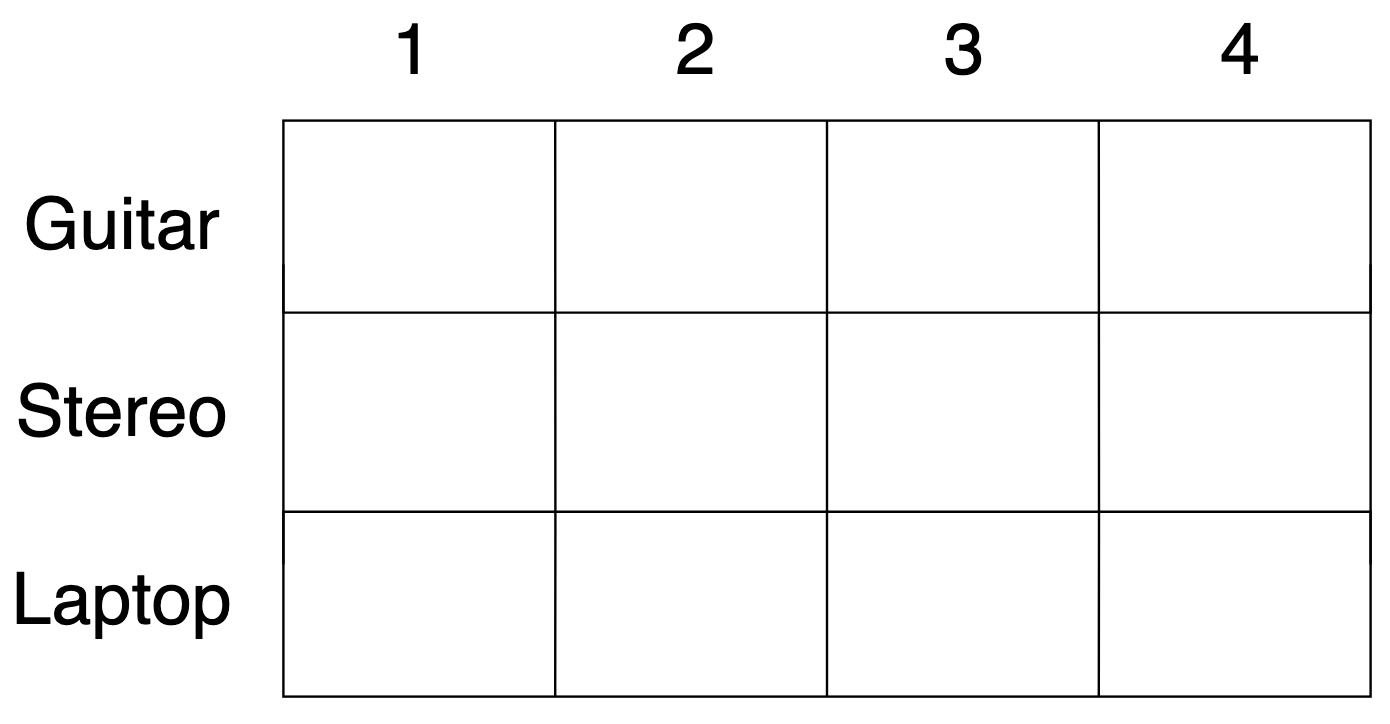
\includegraphics{images/dynamic.png}
\end{column}
\end{columns}
\end{frame}

\begin{frame}{Stereo Row}
\protect\hypertarget{stereo-row}{}
\begin{columns}[T]
\begin{column}{0.5\textwidth}
\begin{itemize}
\item
  In the second row, we can steal the stereo or the guitar.
\item
  At 1 kg, you can only steal the guitar, same as for every other cell
  until Stereo 4, at which point you can steal the stereo and only the
  stereo.
\end{itemize}
\end{column}

\begin{column}{0.5\textwidth}
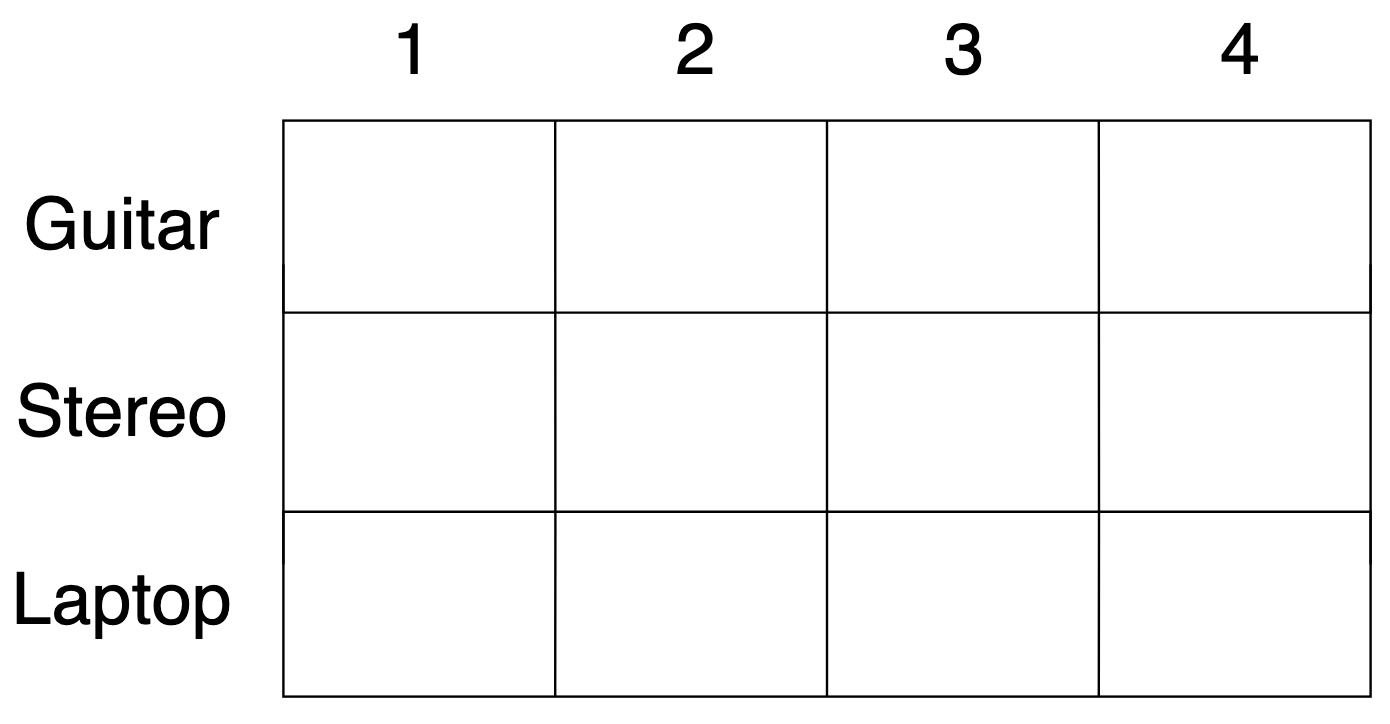
\includegraphics{images/dynamic.png}
\end{column}
\end{columns}
\end{frame}

\begin{frame}{Laptop Row}
\protect\hypertarget{laptop-row}{}
\begin{columns}[T]
\begin{column}{0.5\textwidth}
\begin{itemize}
\item
  Now we can steal all 3 items
\item
  In the first two columns, we still can only steal the guitar. But in
  Laptop 3, we can steal the laptop
\item
  Laptop 4 is the interesting step. We could steal only the stereo, or
  the laptop and something else for 1 kg. What is that 1 kg item?
\item
  According to the above row, the max value for 1 kg is the guitar!
\end{itemize}
\end{column}

\begin{column}{0.5\textwidth}
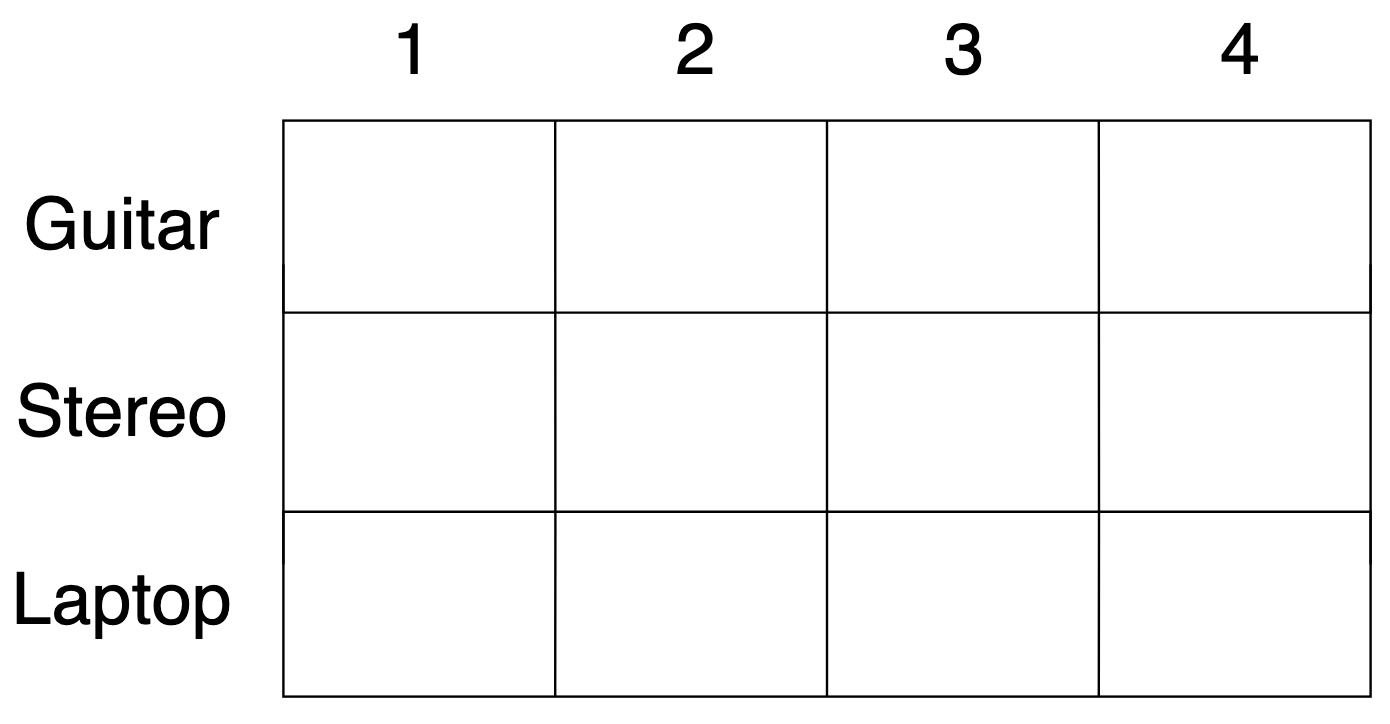
\includegraphics{images/dynamic.png}
\end{column}
\end{columns}
\end{frame}

\begin{frame}{Solution}
\protect\hypertarget{solution}{}
\begin{columns}[T]
\begin{column}{0.5\textwidth}
\begin{itemize}
\item
  If we stole the guitar and laptop, the total value is 3500, which is
  greater than just stealing the stereo
\item
  Thus, we should steal guitar and laptop
\end{itemize}
\end{column}

\begin{column}{0.5\textwidth}
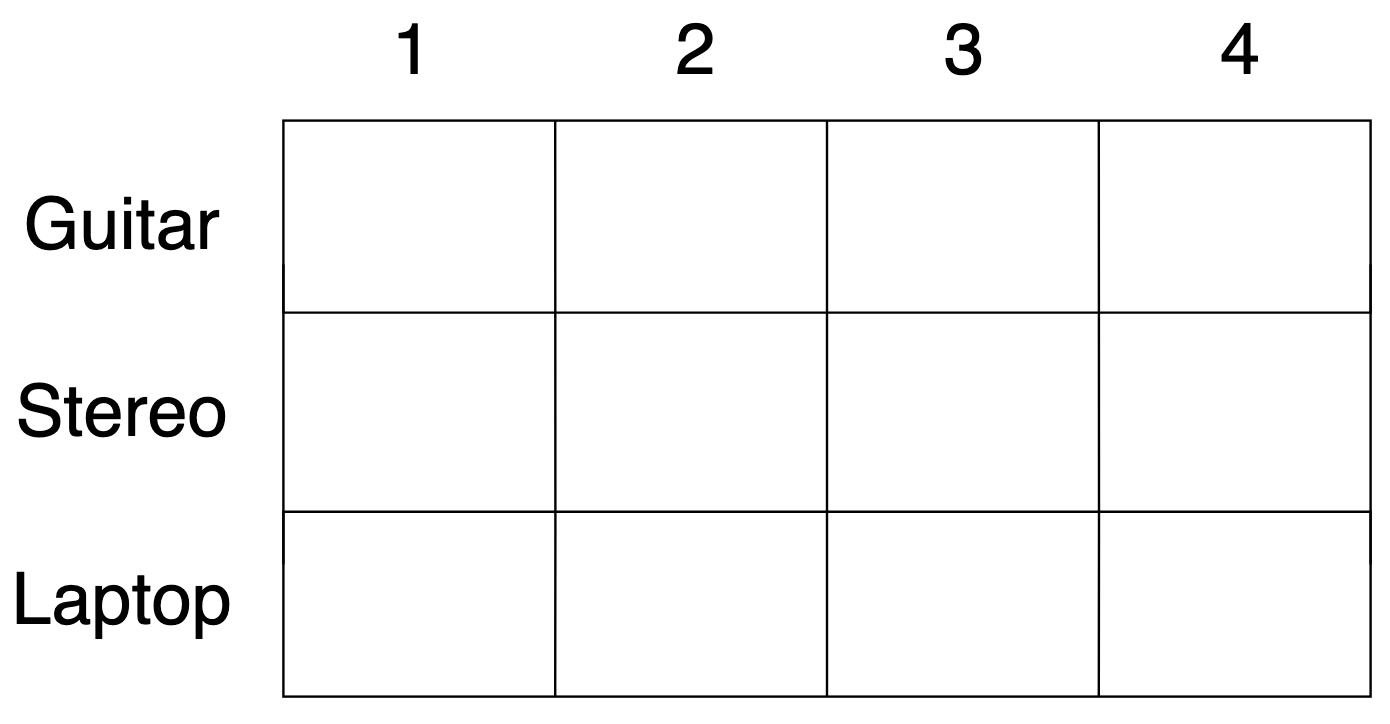
\includegraphics{images/dynamic.png}
\end{column}
\end{columns}
\end{frame}

\begin{frame}{Formula for each cell}
\protect\hypertarget{formula-for-each-cell}{}
\begin{itemize}
\item
  We skipped some very trivial steps in calculating cells aside from the
  last one
\item
  Here's the explicit formula to calculate each cell's value
\end{itemize}

Let \(i\) be the row and \(j\) be the column.

\[
\text{cell}[i][j] = \max
    \begin{cases}
        \text{the previous max at cell}[i-1][j]\\
        \text{value of current item + value of remaining space}
    \end{cases}
\]

The value of remaining space is cell{[}i-1{]}{[}j-item's weight{]}
\end{frame}

\begin{frame}[fragile]{Python Implementation}
\protect\hypertarget{python-implementation}{}
\begin{Shaded}
\begin{Highlighting}[]
\KeywordTok{def}\NormalTok{ initialize\_table(rows, cols):}
  \ControlFlowTok{return}\NormalTok{ [[}\DecValTok{0}\NormalTok{] }\OperatorTok{*}\NormalTok{ cols }\ControlFlowTok{for}\NormalTok{ \_ }\KeywordTok{in} \BuiltInTok{range}\NormalTok{(rows)]}
\end{Highlighting}
\end{Shaded}
\end{frame}

\begin{frame}[fragile]{Python Implementation}
\protect\hypertarget{python-implementation-1}{}
\begin{Shaded}
\begin{Highlighting}[]
\KeywordTok{def}\NormalTok{ knapsack\_dynamic\_programming(values, weights, capacity):}
\NormalTok{  n }\OperatorTok{=} \BuiltInTok{len}\NormalTok{(values)}
\NormalTok{  dp }\OperatorTok{=}\NormalTok{ initialize\_table(n }\OperatorTok{+} \DecValTok{1}\NormalTok{, capacity }\OperatorTok{+} \DecValTok{1}\NormalTok{)}

  \CommentTok{\# Fill the table using dynamic programming}
  \ControlFlowTok{for}\NormalTok{ i }\KeywordTok{in} \BuiltInTok{range}\NormalTok{(}\DecValTok{1}\NormalTok{, n }\OperatorTok{+} \DecValTok{1}\NormalTok{):}
    \ControlFlowTok{for}\NormalTok{ w }\KeywordTok{in} \BuiltInTok{range}\NormalTok{(capacity }\OperatorTok{+} \DecValTok{1}\NormalTok{):}
      \CommentTok{\# Include the current item if it fits in the knapsack}
      \ControlFlowTok{if}\NormalTok{ weights[i }\OperatorTok{{-}} \DecValTok{1}\NormalTok{] }\OperatorTok{\textless{}=}\NormalTok{ w:}
\NormalTok{        dp[i][w] }\OperatorTok{=} \BuiltInTok{max}\NormalTok{(dp[i }\OperatorTok{{-}} \DecValTok{1}\NormalTok{][w], }\OperatorTok{\textbackslash{}}
\NormalTok{        values[i }\OperatorTok{{-}} \DecValTok{1}\NormalTok{] }\OperatorTok{+}\NormalTok{ dp[i }\OperatorTok{{-}} \DecValTok{1}\NormalTok{][w }\OperatorTok{{-}}\NormalTok{ weights[i }\OperatorTok{{-}} \DecValTok{1}\NormalTok{]])}
      \ControlFlowTok{else}\NormalTok{:}
\NormalTok{        dp[i][w] }\OperatorTok{=}\NormalTok{ dp[i }\OperatorTok{{-}} \DecValTok{1}\NormalTok{][w]}

\NormalTok{  selected\_items }\OperatorTok{=}\NormalTok{ traceback(dp, values, weights, capacity)}

  \ControlFlowTok{return}\NormalTok{ dp[n][capacity], selected\_items}
\end{Highlighting}
\end{Shaded}
\end{frame}

\begin{frame}[fragile]{Python Implementation}
\protect\hypertarget{python-implementation-2}{}
\begin{Shaded}
\begin{Highlighting}[]
\KeywordTok{def}\NormalTok{ traceback(dp, values, weights, capacity):}
\NormalTok{  selected\_items }\OperatorTok{=}\NormalTok{ []}
\NormalTok{  i, w }\OperatorTok{=} \BuiltInTok{len}\NormalTok{(dp) }\OperatorTok{{-}} \DecValTok{1}\NormalTok{, capacity}

  \ControlFlowTok{while}\NormalTok{ i }\OperatorTok{\textgreater{}} \DecValTok{0} \KeywordTok{and}\NormalTok{ w }\OperatorTok{\textgreater{}} \DecValTok{0}\NormalTok{:}
    \ControlFlowTok{if}\NormalTok{ dp[i][w] }\OperatorTok{!=}\NormalTok{ dp[i }\OperatorTok{{-}} \DecValTok{1}\NormalTok{][w]:}
\NormalTok{      selected\_items.append(i }\OperatorTok{{-}} \DecValTok{1}\NormalTok{)}
\NormalTok{      w }\OperatorTok{{-}=}\NormalTok{ weights[i }\OperatorTok{{-}} \DecValTok{1}\NormalTok{]}
\NormalTok{      i }\OperatorTok{{-}=} \DecValTok{1}

\NormalTok{  selected\_items.reverse()}
  \ControlFlowTok{return}\NormalTok{ selected\_items}
\end{Highlighting}
\end{Shaded}
\end{frame}

\begin{frame}[fragile]{Python Implementation}
\protect\hypertarget{python-implementation-3}{}
\begin{Shaded}
\begin{Highlighting}[]
\NormalTok{values }\OperatorTok{=}\NormalTok{ [}\DecValTok{3000}\NormalTok{, }\DecValTok{2000}\NormalTok{, }\DecValTok{1500}\NormalTok{]}
\NormalTok{weights }\OperatorTok{=}\NormalTok{ [}\DecValTok{4}\NormalTok{, }\DecValTok{3}\NormalTok{, }\DecValTok{1}\NormalTok{]}
\NormalTok{capacity }\OperatorTok{=} \DecValTok{4}

\NormalTok{max\_value, selected\_items }\OperatorTok{=} \OperatorTok{\textbackslash{}}
\NormalTok{knapsack\_dynamic\_programming(values, weights, capacity)}

\BuiltInTok{print}\NormalTok{(}\StringTok{"Maximum value:"}\NormalTok{, max\_value)}
\BuiltInTok{print}\NormalTok{(}\StringTok{"Selected items:"}\NormalTok{, selected\_items)}
\end{Highlighting}
\end{Shaded}

\begin{verbatim}
Maximum value: 3500
Selected items: [1, 2]
\end{verbatim}
\end{frame}

\begin{frame}[fragile]{Live Coding}
\protect\hypertarget{live-coding}{}
Let a substring be \emph{upper-lower} if for every letter of the
alphabet that the string contains, it appears both in uppercase and
lowercase. For example, \texttt{aaA} is upper-lower because it has both
``A'' and ``a.'' \texttt{aAbb} is not upper-lower because it lacks an
upper case ``B.''

Given string, return the longest substring that is \emph{upper-lower.}

\begin{block}{Example}
\protect\hypertarget{example}{}
\begin{Shaded}
\begin{Highlighting}[]
\CommentTok{\# INPUT}
\NormalTok{string }\OperatorTok{=} \StringTok{"AqeQEfa"}
\CommentTok{\# OUTPUT}
\CommentTok{"qeQE"}
\end{Highlighting}
\end{Shaded}
\end{block}
\end{frame}

\hypertarget{recommended-problems-and-references}{%
\section{Recommended Problems and
References}\label{recommended-problems-and-references}}

\begin{frame}{Recommended Problems and Readings}
\protect\hypertarget{recommended-problems-and-readings}{}
\begin{itemize}
\item
  Cormen (highly optional):
\item
  Chapter 14, more advanced dynamic programming
\item
  Chapter 29, more advanced linear programming
\item
  Bhargava: Chapter 9 exercises

  \begin{itemize}
  \item
    9.1, 9.2
  \item
    Read the knapsack problem FAQs on page 171
  \item
    Follow the example about longest common substring on page 178
  \end{itemize}
\end{itemize}
\end{frame}

\begin{frame}[fragile]{Recommended Problems}
\protect\hypertarget{recommended-problems}{}
\begin{itemize}
\item
  Write the code to brute force the diet problem. Compare the run times
  using the \texttt{timeit} library.
\item
  Modify the code from the slide such that there is an upper bound for
  calories and vitamins.
\item
  Page 17 of Bhargava covered the travelling sales person problem. Is it
  possible to improve the proposed solution using any method we learned
  today?
\end{itemize}
\end{frame}

\begin{frame}{References}
\protect\hypertarget{references}{}
\begin{itemize}
\item
  Bhargava, A. Y. (2016). \emph{Grokking algorithms: An illustrated
  guide for programmers and other curious people.} Manning. Chapter 1.
\item
  Cormen, T. H. (Ed.). (2009). \emph{Introduction to algorithms} (3rd
  ed). MIT Press. Chapter 1 and 3.
\end{itemize}
\end{frame}



\end{document}
